\structure{ХОД РАБОТЫ}

Для решения данной лабораторной работы был использован язык программирования Go.
В проекте был написан класс для решения матричных игр разными способами (аналитическим
и Брауна--Робинсон соответственно). На вход программе подается файл формата JSON с матрицой.

Пример запуска программы:

\begin{codelisting}[language=Bash]
    go run cmd/lw1/main.go tasks/lw1/task.json
\end{codelisting}

Для данной задачи была построена игровая матрица с расчитанными минимальным выигрышом игрока
A и максимальным проигрышем игрока B.

\begin{figure}
  \centering
  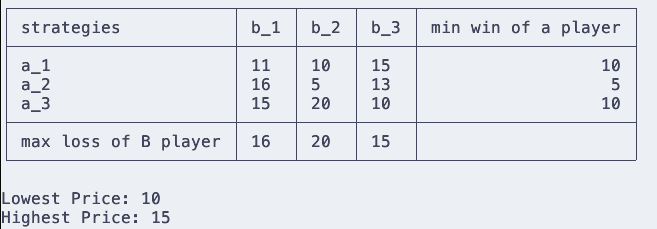
\includegraphics[scale=0.7]{../../artifacts/lw1/game_matrix.png}
  \caption{Вывод игровой матрицы}
  \label{fig:fig01}
\end{figure}

Как видно на рисунке~\ref{fig:fig01}, нижняя цена игры не совпадает с верхней, что говорит об
отсутствии седловой точки.

Перейдем к аналитическому методу решения данной игры.
